\section{Analysis and Design}

In this chapter, the aims are to:

\begin{itemize}
    \item Provide a high-level overview of the design of the system to estimate blood pressure values from PPG signals
    \item Describe the specifications of each stage of the system based on the findings of the literature review in Chapter 2
    \item Discuss any changes or justifications for design choices made for the system blocks where appropriate
\end{itemize}

\subsection{High Level overview of proposed design}
Figure \ref{blockdiag} illustrates the high-level design specification for the 
cuffless estimation of blood pressure from PPG signals. The diagram describes 
each discrete stage that is required. 

\begin{figure}[H]
    \centering
    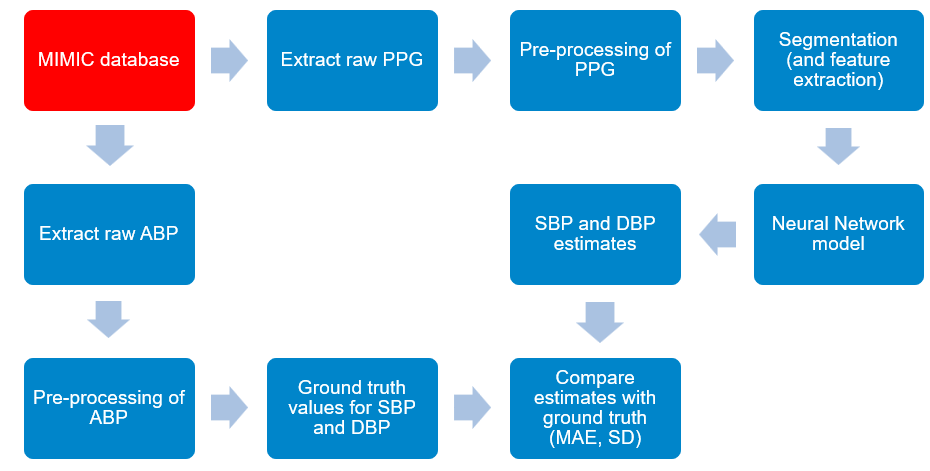
\includegraphics[width=15cm,height=15cm,keepaspectratio]{AnalysisDesign/blockDiag.png}
    \caption{High-level block diagram of blood pressure cuffless estimation from PPG}
    \label{blockdiag}
\end{figure}\noindent The following subchapters will explain each stage in more detail.

\subsection{Choice of database}
As previously discussed in the literature review in Chapter 2, the 
MIMIC (Multi-parameter Intelligent Monitoring for Intensive Care) database has been chosen 
for the implementation. The data has been recorded from patient monitors in the medical, 
surgical, and cardiac intensive care units of Boston's Beth Israel Hospital. The MIMIC Database 
has records for 72 ICU patients. Referring back to the motivation for this FYP, the early detection and prevention of hypertension and other Cardiovascular diseases (CVDs) is 
crucial. Therefore, testing was only performed on patients with CVDs or heart-related issues, which was a data subset of 12 patients. The age range of the patients 
is 52 to 85 years. In addition, the data is from 8 males and 4 females. The data obtained from the bedside monitors are divided into files 
each containing 10 minutes of recorded signals, which can then be assembled without 
gaps to form a continuous recording \cite{Moody1996}. Both the PPG and ABP signals in the MIMIC database 
are sampled at a frequency of $125$ Hz. Each patient record contains a minimum of 73 and a maximum of 412 individual files.
 The patients contain one of the following heart-related diseases:
\begin{itemize}
    \item \textbf{Congestive Heart Failure} (CHF). This refers to patients who suffer a chronic progressive condition that affects the pumping power of your heart muscle \cite{chf}
    \item \textbf{Postoperative Coronary Artery Bypass Graft} (CABG). This refers to patients recovering from a surgical procedure to restore normal blood flow to an obstructed coronary artery \cite{cabg}
    \item \textbf{Myocardial Infarction} (MI) / \textbf{Cardiogenic shock}. This refers to patients who have suffered heart attacks or cardiac shock \cite{mi}
\end{itemize}


\subsection{Choice of programming language}
Python is used as the sole programming language for this project. Python has a wide 
variety of easy to use and powerful libraries \cite{Python}. The scientific libraries from Python 
that are used for this project are \texttt{numpy} \cite{numpy} and \texttt{pandas} \cite{pandas}. In addition, the 
machine learning libraries used are \texttt{tensorflow} \cite{tensorflow}, \texttt{keras} \cite{keras} and \texttt{scikit-learn} \cite{scikit}. 
In addition the \texttt{heartpy} \cite{heartpy} and \texttt{wfdb-python} \cite{wfdb} packages were installed, which are libraries of 
tools for reading, writing, and processing Waveform-Database (WFDB) signals and annotations. For this FYP, Python will be used in the Google Colaboratory environment in the form of a Jupyter notebook, as there is access to 
to high-performance Graphics Processing Units (GPUs) on Google Cloud for training using machine learning.  \\ \newline \noindent MATLAB was also 
considered as a potential programming language to use, due to it having a wide range of 
signal processing and machine learning add-on toolboxes. However Python has been shown 
to offer a wider set of choices in graphics packages and toolsets, such as 
through \texttt{matplotlib} \cite{matplotlib}, and it also produces more compact and readable 
code. 


\subsection{Extraction of raw signal data}
For this implementation, it is necessary to extract the raw signal data 
for two signals, the ABP and PPG. Both signals are first extracted from 
the Physionet website using the \texttt{wfdb} Python package. In order to extract the ground 
truth values for Systolic and Diastolic blood pressure, the following steps are applied to the ABP signal (more detail is provided in Chapter 4):

\begin{itemize}
    \item Use the Python \texttt{heartpy} library to perform sanity checks on the ABP signal (and the PPG) to check whether data can be accurately acquired 
    \item Use a peak detection algorithm to find the Systolic and Diastolic BP and to perform sanity checks on these values
\end{itemize}\noindent These steps are described in more detail in Chapter 4.


\subsection{Pre-processing of PPG}
The PPG signals from the Physionet database need to first be cleaned in order to be analysed accurately. The following steps describe how the PPG signal is pre-processed.
\begin{itemize}
    \item Apply a 4th order Butterworth bandpass filter
    \item Apply Z-score normalisation in order to standardise the data
    \item Additional sanity checks using SBP and DBP minimum and maximum threshold values
\end{itemize}

\subsection{Segmentation (and feature extraction)}
Based on the findings of the literature review, the most recent machine learning methods are favouring automated feature extraction from signal 
data. As a result, the PPG signal itself will be split up, or segmented, into windows of 1 second, and each of these data windows will 
act as input to the neural network model. In addition, the literature review also suggests that there is still high performance among the machine 
learning methods which use handcrafted features. Therefore, as the aim is to assess the performance of the transformer encoder for cuffless blood 
pressure estimation, the following features will also be extracted from the PPG signal and fed into the neural network model (alongside the PPG window segment):

\begin{itemize}
    \item First order derivative of the PPG signal window (with respect to time)
    \item Second order derivative of the PPG signal window (with respect to time)
\end{itemize}\noindent The justification for adding these two features to the PPG window segment is that the transformer encoders 
require a large amount of data to perform well. Therefore, this suggests that purely training the neural network model on the features would be 
detrimental to performance.

\subsection{Neural Network models}
The following Neural Network models will be used to estimate cuffless blood pressure values from PPG signals:
\begin{itemize}
    \item AlexNet (Convolutional Neural Network)
    \item ResNet (Convolutional Neural Network)
    \item ResNet with Leave One Subject Out (LOSO) (Convolutional Neural Network)
    \item Bi-directional Long Short Term Memory (Recurrent Neural Network)
    \item Transformer Encoder
\end{itemize}\noindent All models above have been programmed using functions from the \texttt{tensorflow} and \texttt{keras} libraries and all 
code has been provided in the Appendix and on the Github repository. Further details on each of these architectures is provided in Chapter 4.


\subsection{Error metrics}
The error calculation used in this experimentation is the Mean Absolute Error 
(MAE) for both the Systolic and Diastolic blood pressure values. The MAE is considered so that the results can be compared with the official AAMI/ESH regulations for cuffless blood pressure estimation. MAE is defined by the following equation, 
\begin{align}
    MAE &= \frac{1}{N} \sum_{i=1}^N \lvert a_{i_{M}} - b_{i_{M}} \rvert
\end{align}\noindent In the context of BP estimation, $b_{i_{M}}$ and $a_{i_{M}}$ represent the true 
value and BP estimate respectively for the $M$th element of the time sequence.\\ \newline \noindent To conclude this chapter, a high-level specification of the method used to estimate cuffless blood pressure values from PPG signals has been detailed. 
Where appropriate, decisions made for the high-level specification have been based on the findings of the literature review in the 
previous chapter. Hence, now that the method has been discussed at a high-level, it is now necessary 
to discuss this implementation in more detail.

\subsection{Evaluation of error metrics}
In order to assess how well each of the neural network architectures perform in the cuffless estimation of blood pressure 
values, the MAE value produced will be be assessed against the standards set by the Advancement of Medical Instrumentation (AAMI) \cite{aami}: a MAE blood pressure difference of $\le 5$ mmHg with a standard deviation of $\le 8$ mmHg against 
the gold standard reference measurement.
